\section{Locating the Consistency Boundary (RQ1)}
\label{sec:diagnosis}
\subsection{A repair and a regression under the same intervention}
The continuation experiment tests whether a local path change can recover the reference. The RTX intervention changes target continuation from UB2 to UB1 while retaining prefill, draft settings and caller grouping. On 19 exposed HumanEval tasks, the predictor reproduces both native conditions in all 57 repeated complete arrays. HumanEval/15 repairs, /25 regresses and /18 remains divergent, leaving reference agreement at 51/57 in both conditions. The unchanged aggregate conceals opposing task effects, so continuation-only control does not satisfy recovery without regression.

A separately selected 24-task MBPP panel reaches 72/72 prediction/native agreement in each condition, but only 66/72 reference agreement. MBPP/304 remains a divergent 47-ID response while changing token 488 to 481 at zero-based position 33. Accurate prediction of a changed response does not establish reference recovery. We therefore examine retained state and the current call separately.

\subsection{Natural donor state crossed with the current call}
In Figure~\ref{fig:cross}, rows select naturally formed donor states and columns select the current recipe at a shared committed prefix. Horizontal changes expose current-path dependence; vertical changes expose retained-state dependence. The displayed IDs label decisions rather than numerical distances. A change confined to one donor/recipe pairing indicates an interaction. Own-path shams check that restoration itself preserves the native decision.

For RTX, N0 and N1 denote the native baseline and continuation-intervention histories. Four exposed HumanEval probes yield 24 donors, 48 state/current-path forks and 24 shams across repetitions. Donors preserve actual pending state, cache positions and sampler history. The shams pass and forking leaves the original context unchanged. At /15's 13-token cut, either donor gives 9147 under current UB2 and 4199 under UB1 at the third submitted decision (Figure~\ref{fig:cross}A). The local decision follows the current path. At /25's four-token cut, only the N1-donor/current-UB1 cell changes, producing the sequence 271,750,8168 rather than beginning with 1406 (Figure~\ref{fig:cross}B). This is a local interaction between state and path. The selected /18 and /31 cuts are discrete nulls, which do not establish invariance over their remaining trajectories.

\begin{figure*}[t]
\centering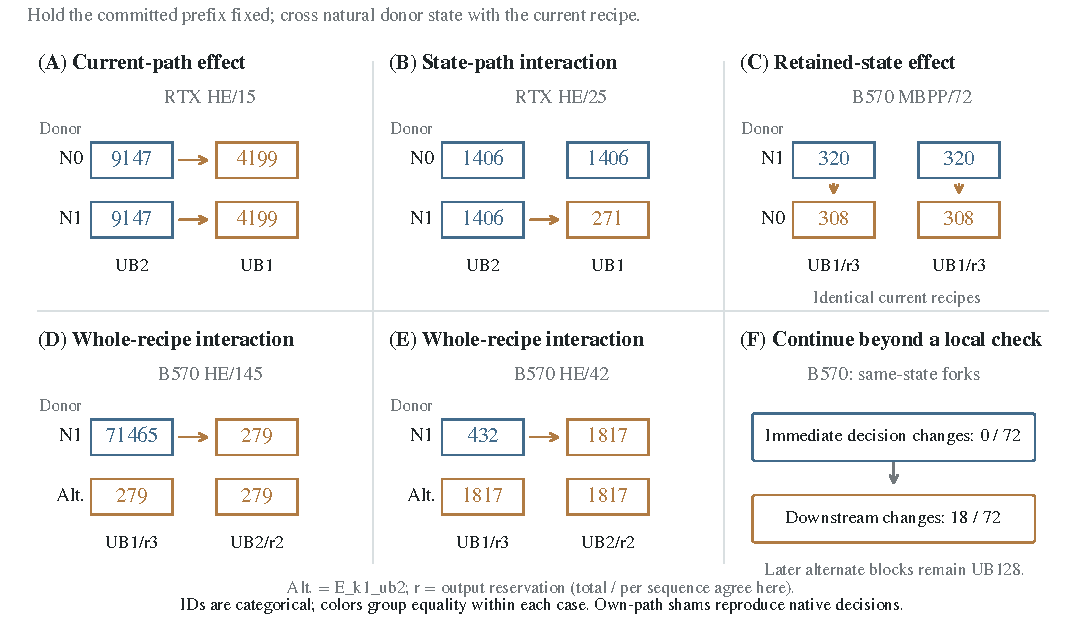
\includegraphics[width=\linewidth]{figures/figure_2_natural_crosses.pdf}
\caption{Three local dependencies and the limit of a local check. Rows select natural donor states; columns select the current recipe. Token IDs are categorical; filled tiles group equal IDs, and links mark equality or difference between adjacent cells. (A) RTX /15 follows the current path. (B) RTX /25 and (D,E) B570 HumanEval show interactions. (C) B570 MBPP/72 follows retained state under identical UB1/reservation3 columns. The B570 HumanEval columns change UB and output reservation together. N0 in (C) is the ordinary donor; Alt. in (D,E) is the cross recipe E\_k1\_ub2. Here $r$ denotes output reservation; the two HumanEval recipes use UB1/$r=3$ and UB2/$r=2$. Own-path shams pass. (F) A separate B570 study finds 0/72 immediate but 18/72 downstream changes under sustained alternate UB128 continuation; it does not isolate a single-block aftereffect.}
\label{fig:cross}
\end{figure*}

All 12 prompt-KV donor comparisons agree, whereas 70 of 72 generated-prefix K/V tensor comparisons differ; the tested first-layer K/V remain equal. The discriminating /15 bonus row is itself a single-token microbatch under either history. Its final nominal shape alone therefore cannot explain the decision: inputs and preceding state formation also matter. The evidence motivates attention-related controls without isolating a unique kernel cause. Auxiliary short continuations and their 1,278 forwards are diagnostic work, not a paid performance panel.

\subsection{One unchanged block does not certify the remaining trajectory}
A separate B570 experiment forks the same live state, with byte-checked KV, at the first eligible verification block after at least 64 committed IDs. It processes that block under UB1 or UB128. Twenty-four reserved prompts and three repetitions produce 72 eligible forks. Every paired raw score record changes, yet immediate top-1 IDs and acceptance decisions remain equal across 195 paired decision events: no execution or task changes its immediate decision.

Complete committed-ID trajectories in Figure~\ref{fig:cross}F differ in 18/72 executions from six of 24 tasks. Later alternate blocks continue to use UB128, and proposals evolve under the accepted history. This result concerns a sustained continuation policy, not one altered block followed by restoration. Qualification must therefore check the registered output beyond the sampled block: a local discrete null can coexist with later divergence, and score movement alone does not predict an immediate decision change. Neither the 72 forks nor the 195 internal events constitute additional independent tasks.

\subsection{B570 crosses identify a whole-recipe boundary}
For B570, N1 labels the repaired prior frontend. The figure labels the alternate HumanEval donor Alt. (E\_k1\_ub2) and the ordinary MBPP/72 donor N0. Neither denotes the later phase-binding candidate. These crosses test whether the RTX diagnostic distinction remains useful in a different runtime. Three tasks in six repeated contexts provide 12 own-path shams and 24 auxiliary target cells. Restored states retain checked byte contents, sequence-zero ownership and logical positions. At HumanEval/145's prefix 56, the selected matrix is $[(71465,279),(279,279)]$; at /42's prefix 73 it is $[(432,1817),(1817,1817)]$ (Figure~\ref{fig:cross}D,E). Both show a local interaction. At MBPP/72's prefix 40, $[(320,320),(308,308)]$ varies only with donor state, under identical current UB1/output-reservation-3 columns (Figure~\ref{fig:cross}C).

The HumanEval recipes change microbatch capacity and output reservation together, so the factor tested is the whole recipe. These crosses do not isolate UB or transfer the RTX repair to Vulkan. Full counterfactual continuations for each cell are unavailable; the subsequent B570 candidate undergoes its own native endpoint qualification. The greedy sampler history, clone metadata and shams support the tested restoration, while opaque sampler bytes and general stochastic-state restoration remain outside that check. At the same committed prefix, local path, state and interaction dependence can require different control placements.

\subsection{Prediction and simple execution constrain added machinery}
Prediction fidelity alone does not establish an online repair mechanism. B570 prospective prediction matches 72/72 native arrays on a reserved 24-task cohort even though reference agreement is 60/72. RTX's initial target-only batched-path predictor reaches 24/36 and fails its frozen 36/36 gate, so no reserved inference follows. A later independent-proposal replay obtains H2/native and reference-only/native agreement of 72/72, again with 60/72 reference agreement. The later study resolves the earlier reproduction interface, but neither result establishes cheap online correction.

On the 19 RTX tasks, draft-free $U_2$ reproduces all 57 intervention $N_1$ arrays and stop boundaries, including /15's repair and /25's regression. It needs no draft, transplant, proposal tape or reference answer. This establishes output equivalence, without a speed claim or demonstrated equality of live logits/KV.

Offline screening provides no supported evidence-acquisition advantage over direct enumeration. RTX direct enumeration and proxy screening both abstain after 114 record equivalents beyond common acquisition; B570 direct verification requires 72 and proxy screening 144. Unknown counterfactuals remain unknown. These are evidence-acquisition counts, not latency measurements. RQ1 identifies local diagnostic distinctions; an automatic repair selector remains unvalidated.
